\documentclass[10pt,aspectratio=169]{beamer}

\usetheme{Madrid}
\usecolortheme{seahorse}
\setbeamertemplate{navigation symbols}{}
\setbeamertemplate{footline}[frame number]

\usepackage[T1]{fontenc}
\usepackage[utf8]{inputenc}
\usepackage{booktabs}
\usepackage{array}
\usepackage{tikz}
\usepackage{xcolor}

\definecolor{deepblue}{RGB}{32,82,149}
\definecolor{softgreen}{RGB}{42,139,93}
\definecolor{warnorange}{RGB}{194,111,38}
\definecolor{lightgray}{RGB}{245,247,250}

\title[Bias Mitigation]{Bias Mitigation in ACSEmployment Prediction}
\subtitle{CS340 Final Project}
\author{Ziheng Wang \and Peizhou Wu}
\date{\today}

\begin{document}

\begin{frame}
  \titlepage
\end{frame}

\begin{frame}{Task and Evaluation Setup}
  \begin{columns}[T,onlytextwidth]
    \begin{column}{0.52\textwidth}
      \begin{block}{Prediction Task}
        \begin{itemize}
          \item Dataset: ACSEmployment, CA and TX, 2018
          \item Target: binary employment status
          \item Sensitive attribute: sex
          \item Held-out evaluation set: 129,383 individuals
        \end{itemize}
      \end{block}
    \end{column}
    \begin{column}{0.43\textwidth}
      \begin{block}{Metric Scope}
        \begin{itemize}
          \item 13 TFMA metrics
          \item 5 extended fairness metrics
          \item Focus: group-level reliability and error gaps
        \end{itemize}
      \end{block}
    \end{column}
  \end{columns}

  \vspace{0.5em}
  \begin{center}
    
\begin{tikzpicture}
      \fill[deepblue!12] (0,0) rectangle (10.8,0.8);
      \node[anchor=west,deepblue] at (0.25,0.4) {Goal: reduce gender-related fairness gaps without losing too much predictive utility.};
    \end{tikzpicture}
  \end{center}
\end{frame}

\begin{frame}[t]{Baseline Metrics by Sex}
  \begin{columns}[T,onlytextwidth]
    \begin{column}{0.49\textwidth}
      \centering
      \resizebox{\linewidth}{!}{%
        \begin{tabular}{|l|c|c|c|}
        \hline
        \textbf{Metric} & \textbf{Female} & \textbf{Male} & \textbf{Overall} \\
        \hline
        \textbf{Sample Size} & 65,819 & 63,564 & 129,383 \\
        \hline
        \textbf{AUC} & 0.8713 & 0.9244 & 0.9016 \\
        \textbf{Binary Accuracy} & 0.7889 & 0.8527 & 0.8202 \\
        \hline
        \textbf{Positive Rate} & 0.4668 & 0.5253 & 0.4956 \\
        \textbf{Negative Rate} & 0.5332 & 0.4747 & 0.5044 \\
        \hline
        \textbf{Precision} & 0.7216 & 0.8267 & 0.7763 \\
        \textbf{Recall (TPR)} & 0.8059 & 0.8853 & 0.8481 \\
        \textbf{True Negative Rate} & 0.7767 & 0.8213 & 0.7971 \\
        \hline
        \textbf{False Positive Rate} & 0.2233 & 0.1787 & 0.2029 \\
        \textbf{False Negative Rate} & 0.1941 & 0.1147 & 0.1519 \\
        \textbf{False Discovery Rate} & 0.2784 & 0.1733 & 0.2237 \\
        \textbf{False Omission Rate} & 0.1521 & 0.1186 & 0.1366 \\
        \hline
        \end{tabular}%
      }
      \vspace{0.4em}
      {\footnotesize Base model performance metrics by sex}
    \end{column}
    \begin{column}{0.49\textwidth}
      \centering
      \resizebox{\linewidth}{!}{%
        \begin{tabular}{|l|c|c|c|}
        \hline
        \textbf{Fairness Metric} & \textbf{Value/Difference} & \textbf{Threshold} & \textbf{Status} \\
        \hline
        \textbf{Disparate Impact (80\% Rule)} &  &  &  \\
        \quad Female Positive Rate & 0.4668 &  &  \\
        \quad Male Positive Rate & 0.5253 &  &  \\
        \quad Ratio & 0.8886 & $\geq 0.80$ & Fair  \\
        \hline
        \textbf{Average Odds Difference} & 0.0620 & $\leq 0.10$ & Fair  \\
        \hline
        \textbf{Predictive Parity} &  &  &  \\
        \quad Female Precision & 0.7216 &  &  \\
        \quad Male Precision & 0.8267 &  &  \\
        \quad Difference & 0.1051 & $\leq 0.10$ & Unfair \\
        \hline
        \textbf{NPV Equality (Cond. Use Accuracy)} &  &  &  \\
        \quad Female NPV & 0.8479 &  &  \\
        \quad Male NPV & 0.8814 &  &  \\
        \quad Difference & 0.0335 & $\leq 0.10$ & Fair \\
        \hline
        \textbf{Performance Gaps (AUC)} &  &  &  \\
        \quad Female AUC & 0.8713 &  &  \\
        \quad Male AUC & 0.9244 &  &  \\
        \quad AUC Gap & 0.0531 & $\leq 0.05$ & Unfair  \\
        \hline
        \end{tabular}%
      }
      \vspace{0.4em}
      {\footnotesize Base model extended fairness metrics summary}
    \end{column}
  \end{columns}
\end{frame}

\begin{frame}{Baseline Bias Pattern}
  \begin{columns}[T,onlytextwidth]
    \begin{column}{0.48\textwidth}
      \begin{block}{What the Baseline Gets Right}
        \begin{itemize}
          \item Disparate Impact is within the 80\% rule: $0.8886$
          \item Average Odds Difference is acceptable: $0.0620$
          \item NPV Equality is also within threshold: $0.0335$
        \end{itemize}
      \end{block}

      \begin{alertblock}{Main Takeaway}
        The baseline is not uniformly unfair; the largest issues are concentrated in prediction reliability and ranking.
      \end{alertblock}
    \end{column}
    \begin{column}{0.48\textwidth}
      \begin{block}{Where the Gaps Remain}
        \begin{itemize}
          \item Predictive Parity gap: $0.1051$ \;($>$ 0.10 threshold)
          \item AUC gap: $0.0531$ \;($>$ 0.05 threshold)
          \item Female precision is lower than male: $0.7216$ vs. $0.8267$
        \end{itemize}
      \end{block}

      \begin{exampleblock}{Error Pattern}
        Female FPR and FNR are both higher than male: $0.2233$ vs. $0.1787$ and $0.1941$ vs. $0.1147$.
      \end{exampleblock}
    \end{column}
  \end{columns}

  \vspace{0.3em}
  \begin{center}
    
\begin{tikzpicture}
      \fill[warnorange!12] (0,0) rectangle (11.0,0.75);
      \node[anchor=west,warnorange] at (0.25,0.38) {Mitigation should target error-rate parity and representation bias, not just positive rate balance.};
    \end{tikzpicture}
  \end{center}
\end{frame}

\begin{frame}{Mitigation Method}
  \begin{columns}[T,onlytextwidth]
    \begin{column}{0.32\textwidth}
      \begin{block}{1. Adversarial Debiasing}
        Gradient reversal discourages gender information in hidden representations.
      \end{block}
    \end{column}
    \begin{column}{0.32\textwidth}
      \begin{block}{2. Equalized Odds Loss}
        Directly penalizes FNR and FPR differences across groups.
      \end{block}
    \end{column}
    \begin{column}{0.32\textwidth}
      \begin{block}{3. Sample Re-weighting}
        Balances gender groups and boosts positive examples by 1.5x.
      \end{block}
    \end{column}
  \end{columns}

  \vspace{1.0em}
  \begin{equation*}
    \mathcal{L}_{main} = \mathcal{L}_{BCE}(y,\hat{y})
    + \lambda_{fair}\left(|FNR_f-FNR_m| + |FPR_f-FPR_m|\right)
  \end{equation*}
  \vspace{-0.4em}
  \begin{center}
    $\lambda_{adv}=0.5,\quad \lambda_{fair}=0.5,\quad$ Adam optimizer, 25 epochs
  \end{center}
\end{frame}

\begin{frame}[t]{Double-Win Scorecard}
  \centering
  \resizebox{0.63\textwidth}{!}{%
    \begin{tabular}{|l|cc|cc|c|}
    \hline
    \textbf{Metric} &
    \textbf{Base F} & \textbf{Fair F} &
    \textbf{Base M} & \textbf{Fair M} &
    \textbf{Result} \\
    \hline
    \multicolumn{6}{|l|}{\textit{Auto-pass (teacher policy)}} \\
    \hline
    Example Count & 65{,}819 & 66{,}809 & 63{,}564 & 62{,}574 & \textbf{WIN} \\
    \hline
    \multicolumn{6}{|l|}{\textit{Double wins -- both groups improve}} \\
    \hline
    False Negative Rate   & 0.1887 & \textbf{0.0814} & 0.1139 & \textbf{0.0666} & \textbf{WIN} \\
    False Omission Rate   & 0.1488 & \textbf{0.0816} & 0.1180 & \textbf{0.0830} & \textbf{WIN} \\
    Negative Rate         & 0.5302 & \textbf{0.4165} & 0.4735 & \textbf{0.3936} & \textbf{WIN} \\
    Positive Rate         & 0.4698 & \textbf{0.5835} & 0.5265 & \textbf{0.6064} & \textbf{WIN} \\
    Recall (TPR)          & 0.8113 & \textbf{0.9186} & 0.8861 & \textbf{0.9334} & \textbf{WIN} \\
    True Positive Rate    & 0.8113 & \textbf{0.9186} & 0.8861 & \textbf{0.9334} & \textbf{WIN} \\
    \hline
    \multicolumn{6}{|l|}{\textit{Double losses -- both groups regress}} \\
    \hline
    AUC                   & \textbf{0.8716} & 0.8615 & \textbf{0.9242} & 0.8994 & LOSS \\
    Binary Accuracy       & \textbf{0.7903} & 0.7665 & \textbf{0.8523} & 0.8188 & LOSS \\
    False Discovery Rate  & \textbf{0.2784} & 0.3420 & \textbf{0.1744} & 0.2449 & LOSS \\
    False Positive Rate   & \textbf{0.2247} & 0.3428 & \textbf{0.1803} & 0.2915 & LOSS \\
    Precision             & \textbf{0.7216} & 0.6580 & \textbf{0.8256} & 0.7551 & LOSS \\
    True Negative Rate    & \textbf{0.7753} & 0.6572 & \textbf{0.8197} & 0.7085 & LOSS \\
    \hline
    \multicolumn{4}{|l|}{\textbf{Total Double Wins}} &
    \multicolumn{2}{c|}{\textbf{7 / 13}} \\
    \hline
    \end{tabular}%
  }
\end{frame}

\begin{frame}{Extended Fairness Metrics Improved}
  \begin{table}
    \small
    \begin{tabular}{lccc}
      \toprule
      Metric & Base Model & Fair Model & Direction \\
      \midrule
      Disparate Impact Ratio & 0.8886 & 0.9622 & closer to 1 \\
      Average Odds Difference & 0.0620 & 0.0330 & lower \\
      Predictive Parity Gap & 0.1051 & 0.0971 & lower \\
      NPV Equality Gap & 0.0335 & 0.0014 & lower \\
      AUC Gap & 0.0531 & 0.0378 & lower \\
      \bottomrule
    \end{tabular}
  \end{table}

  \vspace{0.8em}
  \begin{center}
    
\begin{tikzpicture}
      \fill[softgreen!12] (0,0) rectangle (11.4,0.85);
      \node[anchor=west,softgreen] at (0.25,0.43) {All five extended fairness metrics move in the desired direction.};
    \end{tikzpicture}
  \end{center}
\end{frame}


\begin{frame}{Overall Experimental Result}
  \begin{columns}[T,onlytextwidth]
    \begin{column}{0.47\textwidth}
      \begin{block}{Improved Metrics}
        \begin{itemize}
          \item 12 metrics improved in total
          \item 5 extended fairness metrics improved
          \item 7 TFMA metrics improved
        \end{itemize}
      \end{block}
    \end{column}
    
  \end{columns}

  \vspace{0.8em}
  \begin{center}
    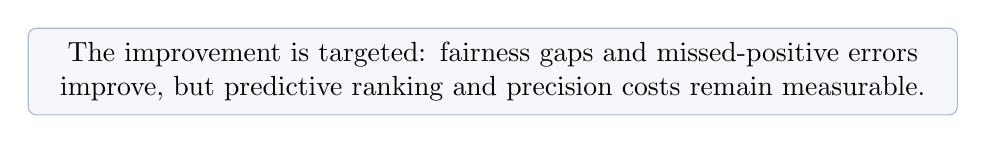
\begin{tikzpicture}
      \draw[rounded corners=3pt,fill=lightgray,draw=deepblue!40] (0,0) rectangle (11.8,1.1);
      \node[text width=11.1cm,align=center] at (5.9,0.55)
      {The improvement is targeted: fairness gaps and missed-positive errors improve, but predictive ranking and precision costs remain measurable.};
    \end{tikzpicture}
  \end{center}
\end{frame}

\begin{frame}{Performance Trade-off}
  \begin{columns}[T,onlytextwidth]
    \begin{column}{0.52\textwidth}
      \begin{table}
        \small
        \begin{tabular}{lccc}
          \toprule
          Metric & Base & Fair & Change \\
          \midrule
          AUC & 0.9016 & 0.8784 & -0.0232 \\
          Accuracy & 0.8202 & 0.7922 & -0.0280 \\
          Precision & 0.7763 & 0.7066 & -0.0697 \\
          Recall / TPR & 0.8481 & 0.9265 & +0.0784 \\
          FNR & 0.1519 & 0.0735 & -0.0784 \\
          FPR & 0.2029 & 0.3193 & +0.1164 \\
          \bottomrule
        \end{tabular}
      \end{table}
    \end{column}
    \begin{column}{0.44\textwidth}
      \begin{block}{Interpretation}
        \begin{itemize}
          \item The model predicts more positives after mitigation.
          \item Fewer positive cases are missed.
          \item More false positives are introduced.
        \end{itemize}
      \end{block}
      \begin{alertblock}{Main Trade-off}
        Fairness and recall improve, while accuracy, AUC, and precision decrease.
      \end{alertblock}
    \end{column}
  \end{columns}
\end{frame}



\begin{frame}{Conclusion}
  \begin{itemize}
    \item Adversarial debiasing, Equalized Odds loss, and sample re-weighting improve all five extended fairness metrics.
    \item The fair model reduces the AUC gap from 0.0531 to 0.0378 and predictive parity gap from 0.1051 to 0.0971.
    \item Recall improves from 0.8481 to 0.9265, reducing missed positive cases.
    \item Accuracy, AUC, precision, and FPR show that fairness gains come with real performance trade-offs.
  \end{itemize}

  \vfill
  \begin{center}
    \Large Questions?
  \end{center}
\end{frame}

\end{document}
